% Created by tikzDevice version 0.12.5 on 2023-11-24 23:42:35
% !TEX encoding = UTF-8 Unicode
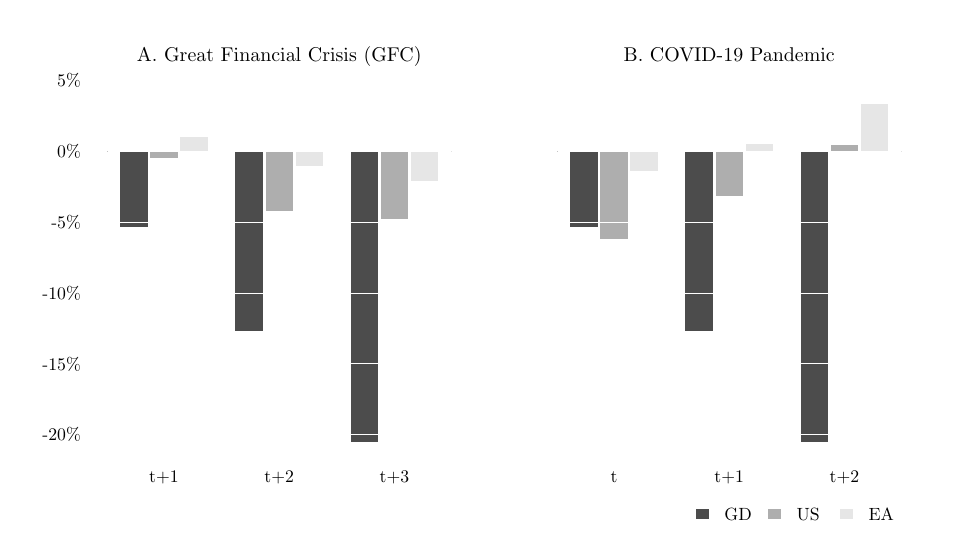
\begin{tikzpicture}[x=1pt,y=1pt]
\definecolor{fillColor}{RGB}{255,255,255}
\path[use as bounding box,fill=fillColor,fill opacity=0.00] (0,0) rectangle (325.21,180.67);
\begin{scope}
\path[clip] (  0.00,  0.00) rectangle (162.61,180.67);
\definecolor{fillColor}{gray}{0.30}

\path[fill=fillColor] ( 33.40,135.90) rectangle ( 43.31,108.47);
\definecolor{fillColor}{RGB}{174,174,174}

\path[fill=fillColor] ( 44.31,135.90) rectangle ( 54.22,133.50);
\definecolor{fillColor}{RGB}{230,230,230}

\path[fill=fillColor] ( 55.21,135.90) rectangle ( 65.13,141.05);
\definecolor{fillColor}{gray}{0.30}

\path[fill=fillColor] ( 75.04,135.90) rectangle ( 84.96, 70.99);
\definecolor{fillColor}{RGB}{174,174,174}

\path[fill=fillColor] ( 85.95,135.90) rectangle ( 95.86,114.29);
\definecolor{fillColor}{RGB}{230,230,230}

\path[fill=fillColor] ( 96.85,135.90) rectangle (106.77,130.64);
\definecolor{fillColor}{gray}{0.30}

\path[fill=fillColor] (116.68,135.90) rectangle (126.60, 30.87);
\definecolor{fillColor}{RGB}{174,174,174}

\path[fill=fillColor] (127.59,135.90) rectangle (137.50,111.44);
\definecolor{fillColor}{RGB}{230,230,230}

\path[fill=fillColor] (138.49,135.90) rectangle (148.41,125.35);
\end{scope}
\begin{scope}
\path[clip] (  0.00,  0.00) rectangle (325.21,180.67);
\definecolor{drawColor}{RGB}{0,0,0}

\node[text=drawColor,anchor=base,inner sep=0pt, outer sep=0pt, scale=  0.64] at ( 49.26, 16.32) {t+1};

\node[text=drawColor,anchor=base,inner sep=0pt, outer sep=0pt, scale=  0.64] at ( 90.90, 16.32) {t+2};

\node[text=drawColor,anchor=base,inner sep=0pt, outer sep=0pt, scale=  0.64] at (132.54, 16.32) {t+3};
\end{scope}
\begin{scope}
\path[clip] ( 28.80, 33.60) rectangle (153.01,161.47);
\definecolor{drawColor}{RGB}{0,0,0}

\path[draw=drawColor,line width= 0.4pt,line join=round,line cap=round] ( 28.80,135.90) -- (153.01,135.90);
\end{scope}
\begin{scope}
\path[clip] (  0.00,  0.00) rectangle (325.21,180.67);
\definecolor{drawColor}{RGB}{0,0,0}

\node[text=drawColor,anchor=base east,inner sep=0pt, outer sep=0pt, scale=  0.64] at ( 19.20, 31.40) {-20\%};

\node[text=drawColor,anchor=base east,inner sep=0pt, outer sep=0pt, scale=  0.64] at ( 19.20, 56.97) {-15\%};

\node[text=drawColor,anchor=base east,inner sep=0pt, outer sep=0pt, scale=  0.64] at ( 19.20, 82.55) {-10\%};

\node[text=drawColor,anchor=base east,inner sep=0pt, outer sep=0pt, scale=  0.64] at ( 19.20,108.12) {-5\%};

\node[text=drawColor,anchor=base east,inner sep=0pt, outer sep=0pt, scale=  0.64] at ( 19.20,133.70) {0\%};

\node[text=drawColor,anchor=base east,inner sep=0pt, outer sep=0pt, scale=  0.64] at ( 19.20,159.27) {5\%};
\end{scope}
\begin{scope}
\path[clip] ( 28.80, 33.60) rectangle (153.01,161.47);
\definecolor{drawColor}{RGB}{255,255,255}

\path[draw=drawColor,line width= 0.4pt,line join=round,line cap=round] ( 28.80, 33.60) -- (153.01, 33.60);

\path[draw=drawColor,line width= 0.4pt,line join=round,line cap=round] ( 28.80, 59.17) -- (153.01, 59.17);

\path[draw=drawColor,line width= 0.4pt,line join=round,line cap=round] ( 28.80, 84.75) -- (153.01, 84.75);

\path[draw=drawColor,line width= 0.4pt,line join=round,line cap=round] ( 28.80,110.33) -- (153.01,110.33);

\path[draw=drawColor,line width= 0.4pt,line join=round,line cap=round] ( 28.80,135.90) -- (153.01,135.90);

\path[draw=drawColor,line width= 0.4pt,line join=round,line cap=round] ( 28.80,161.47) -- (153.01,161.47);
\end{scope}
\begin{scope}
\path[clip] (  0.00,  0.00) rectangle (162.61,180.67);
\definecolor{drawColor}{RGB}{0,0,0}

\node[text=drawColor,anchor=base,inner sep=0pt, outer sep=0pt, scale=  0.72] at ( 90.90,168.60) {A. Great Financial Crisis (GFC)};
\end{scope}
\begin{scope}
\path[clip] (162.61,  0.00) rectangle (325.21,180.67);
\definecolor{fillColor}{gray}{0.30}

\path[fill=fillColor] (196.01,135.90) rectangle (205.92,108.47);
\definecolor{fillColor}{RGB}{174,174,174}

\path[fill=fillColor] (206.91,135.90) rectangle (216.83,104.27);
\definecolor{fillColor}{RGB}{230,230,230}

\path[fill=fillColor] (217.82,135.90) rectangle (227.73,128.84);
\definecolor{fillColor}{gray}{0.30}

\path[fill=fillColor] (237.65,135.90) rectangle (247.56, 70.99);
\definecolor{fillColor}{RGB}{174,174,174}

\path[fill=fillColor] (248.55,135.90) rectangle (258.47,119.80);
\definecolor{fillColor}{RGB}{230,230,230}

\path[fill=fillColor] (259.46,135.90) rectangle (269.37,138.54);
\definecolor{fillColor}{gray}{0.30}

\path[fill=fillColor] (279.29,135.90) rectangle (289.20, 30.87);
\definecolor{fillColor}{RGB}{174,174,174}

\path[fill=fillColor] (290.19,135.90) rectangle (300.11,138.34);
\definecolor{fillColor}{RGB}{230,230,230}

\path[fill=fillColor] (301.10,135.90) rectangle (311.01,152.93);
\end{scope}
\begin{scope}
\path[clip] (  0.00,  0.00) rectangle (325.21,180.67);
\definecolor{drawColor}{RGB}{0,0,0}

\node[text=drawColor,anchor=base,inner sep=0pt, outer sep=0pt, scale=  0.64] at (211.87, 16.32) {t};

\node[text=drawColor,anchor=base,inner sep=0pt, outer sep=0pt, scale=  0.64] at (253.51, 16.32) {t+1};

\node[text=drawColor,anchor=base,inner sep=0pt, outer sep=0pt, scale=  0.64] at (295.15, 16.32) {t+2};
\end{scope}
\begin{scope}
\path[clip] (191.41, 33.60) rectangle (315.62,161.47);
\definecolor{drawColor}{RGB}{0,0,0}

\path[draw=drawColor,line width= 0.4pt,line join=round,line cap=round] (191.41,135.90) -- (315.62,135.90);
\definecolor{drawColor}{RGB}{255,255,255}

\path[draw=drawColor,line width= 0.4pt,line join=round,line cap=round] (191.41, 33.60) -- (315.62, 33.60);

\path[draw=drawColor,line width= 0.4pt,line join=round,line cap=round] (191.41, 59.17) -- (315.62, 59.17);

\path[draw=drawColor,line width= 0.4pt,line join=round,line cap=round] (191.41, 84.75) -- (315.62, 84.75);

\path[draw=drawColor,line width= 0.4pt,line join=round,line cap=round] (191.41,110.33) -- (315.62,110.33);

\path[draw=drawColor,line width= 0.4pt,line join=round,line cap=round] (191.41,135.90) -- (315.62,135.90);

\path[draw=drawColor,line width= 0.4pt,line join=round,line cap=round] (191.41,161.47) -- (315.62,161.47);
\end{scope}
\begin{scope}
\path[clip] (162.61,  0.00) rectangle (325.21,180.67);
\definecolor{fillColor}{gray}{0.30}

\path[fill=fillColor] (241.43,  6.87) rectangle (246.03,  3.03);
\definecolor{fillColor}{RGB}{174,174,174}

\path[fill=fillColor] (267.46,  6.87) rectangle (272.07,  3.03);
\definecolor{fillColor}{RGB}{230,230,230}

\path[fill=fillColor] (293.50,  6.87) rectangle (298.11,  3.03);
\definecolor{drawColor}{RGB}{0,0,0}

\node[text=drawColor,anchor=base west,inner sep=0pt, outer sep=0pt, scale=  0.64] at (251.79,  2.74) {GD};

\node[text=drawColor,anchor=base west,inner sep=0pt, outer sep=0pt, scale=  0.64] at (277.83,  2.74) {US};

\node[text=drawColor,anchor=base west,inner sep=0pt, outer sep=0pt, scale=  0.64] at (303.87,  2.74) {EA};

\node[text=drawColor,anchor=base,inner sep=0pt, outer sep=0pt, scale=  0.72] at (253.51,168.60) {B. COVID-19 Pandemic};
\end{scope}
\end{tikzpicture}
